\documentclass[10pt,twocolumn]{article}

% A compact two-column mockup for checking how the bundled plots read in a paper.
\usepackage[
  paperwidth=8.5in,
  paperheight=11in,
  top=0.62in,
  bottom=0.68in,
  left=0.68in,
  right=0.68in,
  columnsep=0.24in
]{geometry}
\usepackage{graphicx}
\usepackage{microtype}
\usepackage{booktabs}
\usepackage{xcolor}
\usepackage{subcaption}

\definecolor{paperblue}{HTML}{1F4E79}
\captionsetup{
  font=small,
  labelfont=bf,
  labelsep=period,
  skip=4pt
}
\captionsetup[subfigure]{font=footnotesize,labelfont=bf,skip=2pt}
\setlength{\parindent}{1em}
\setlength{\parskip}{0pt}

\title{\vspace{-1.2em}\textbf{A Paper-Layout Preview for Scientific Plots}}
\author{Example Research Group}
\date{}

\begin{document}

\twocolumn[{
  \maketitle
  \vspace{-1.5em}
  \begin{abstract}
  This compact mockup shows how the repository's vector plots look after
  insertion into a conventional two-column paper. It includes a regular
  single-column figure and a full-width figure spanning both columns.
  \end{abstract}
  \vspace{0.8em}
}]

\section{Overview}
Scientific figures are usually judged at their final publication size rather
than at the size used during editing. Figure~\ref{fig:single-column} shows a
typical single-column comparison: two related plots share one caption while
each subfigure keeps its own local label. The text remains readable at the
column width, and the axes do not compete with the caption.

\begin{figure}[t]
  \centering
  \begin{subfigure}[t]{0.485\columnwidth}
    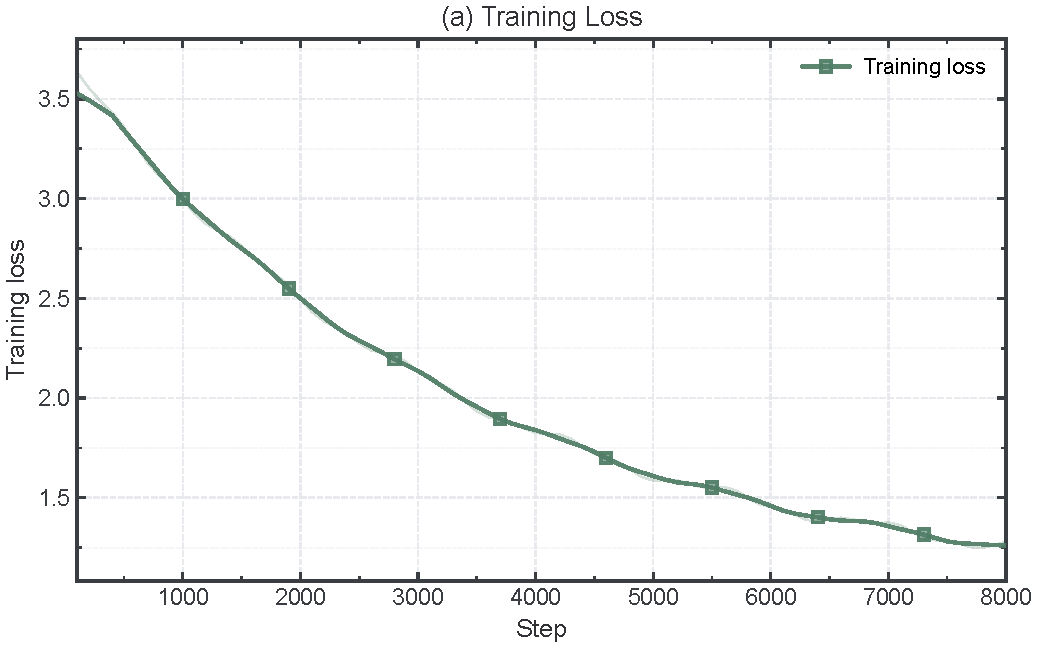
\includegraphics[width=\linewidth]{../sample_llm_training_curves_a_train_loss.pdf}
    \caption{Training loss.}
  \end{subfigure}\hfill
  \begin{subfigure}[t]{0.485\columnwidth}
    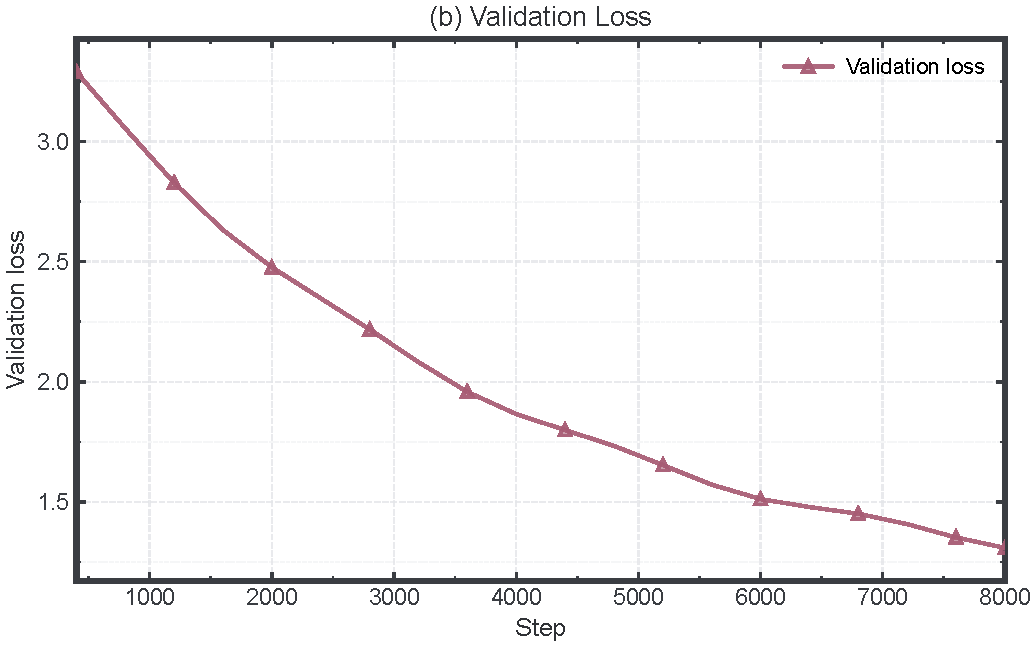
\includegraphics[width=\linewidth]{../sample_llm_training_curves_b_val_loss.pdf}
    \caption{Validation loss.}
  \end{subfigure}
  \caption{A single-column figure with two related learning curves. The
  subfigures are sized against the actual column width rather than an
  arbitrary slide canvas.}
  \label{fig:single-column}
\end{figure}

\section{Experimental setting}
The mockup uses the same PDF assets that are linked in the repository README.
Because the source files are vector PDFs, line weights and labels remain sharp
when the figure is magnified. In practice, this is the point at which overly
small tick labels, long legends, or excessive whitespace become visible.

Table~\ref{tab:settings} gives the kind of compact context that normally
appears next to a figure in a methods or experiments section.

\begin{table}[t]
  \centering
  \caption{Example training configuration.}
  \label{tab:settings}
  \small
  \begin{tabular}{@{}ll@{}}
    \toprule
    Optimizer & AdamW \\
    Batch size & 128 \\
    Warmup steps & 800 \\
    Evaluation interval & 400 steps \\
    \bottomrule
  \end{tabular}
\end{table}

The full-width layout in Figure~\ref{fig:full-width} is useful when four
panels need to be compared together. It also makes the trade-off explicit:
the panels receive more horizontal space, but the figure consumes the full
page width and should therefore carry one focused caption rather than several
independent explanations.

\begin{figure*}[t]
  \centering
  \begin{subfigure}[t]{0.235\textwidth}
    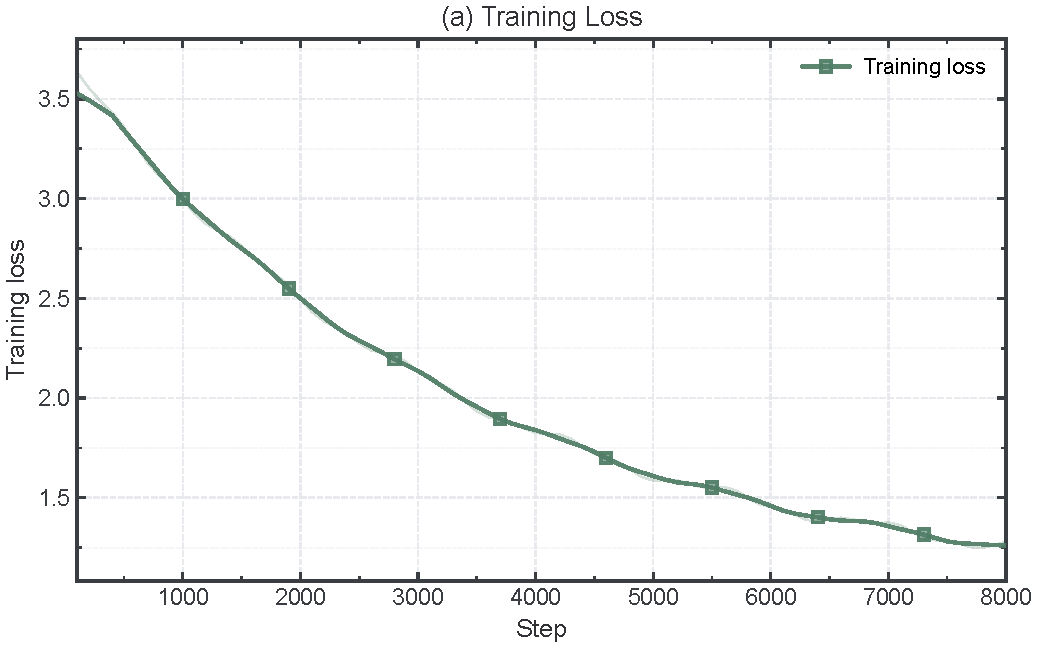
\includegraphics[width=\linewidth]{../sample_llm_training_curves_a_train_loss.pdf}
    \caption{Training loss.}
  \end{subfigure}\hfill
  \begin{subfigure}[t]{0.235\textwidth}
    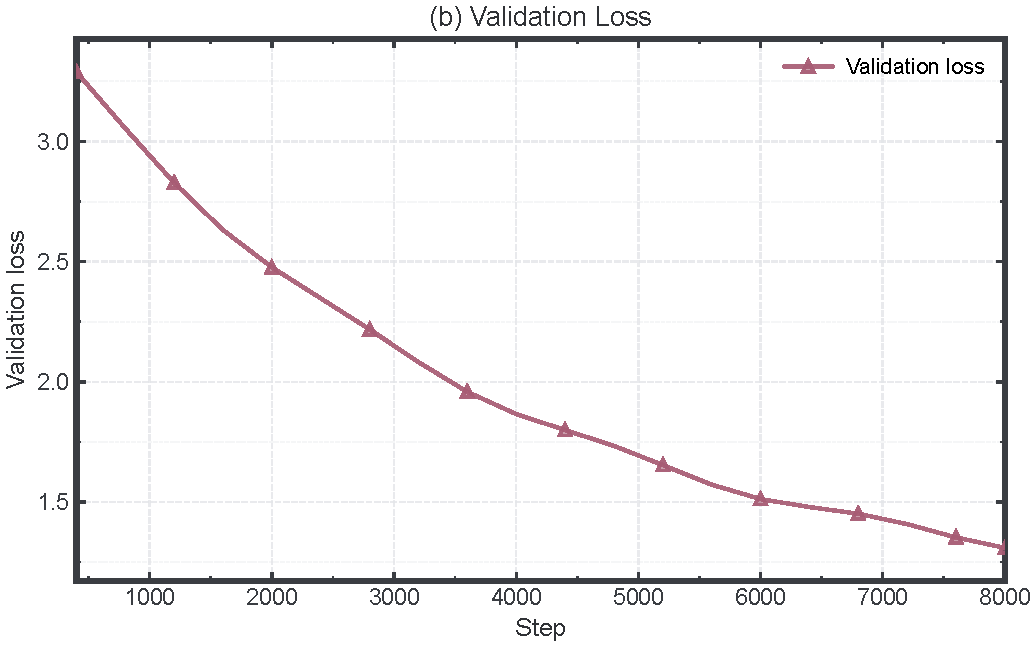
\includegraphics[width=\linewidth]{../sample_llm_training_curves_b_val_loss.pdf}
    \caption{Validation loss.}
  \end{subfigure}\hfill
  \begin{subfigure}[t]{0.235\textwidth}
    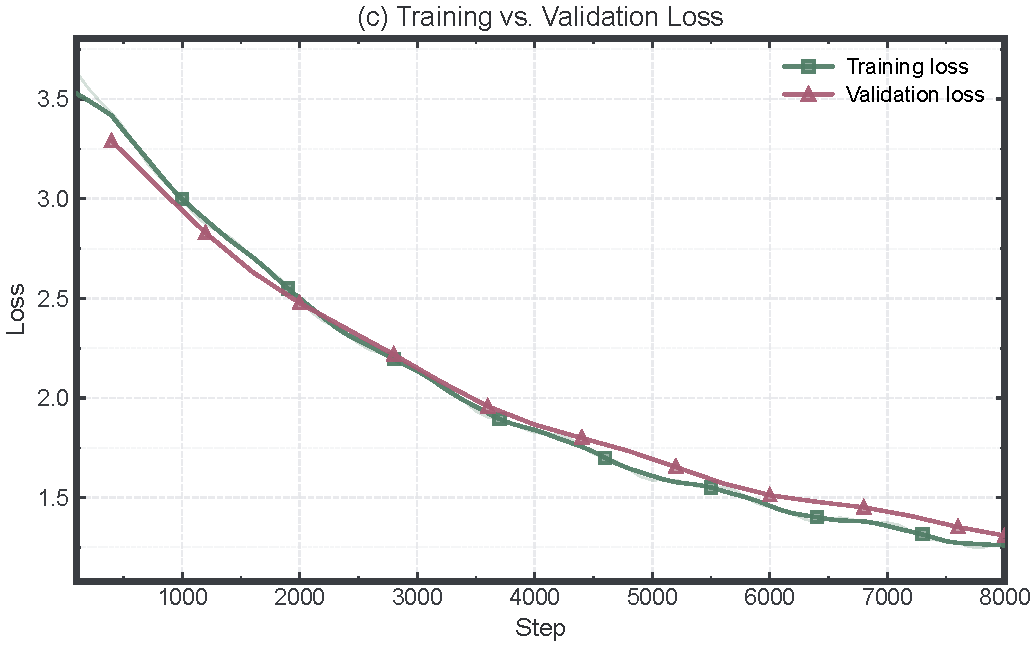
\includegraphics[width=\linewidth]{../sample_llm_training_curves_c_train_vs_val_loss.pdf}
    \caption{Train vs. validation.}
  \end{subfigure}\hfill
  \begin{subfigure}[t]{0.235\textwidth}
    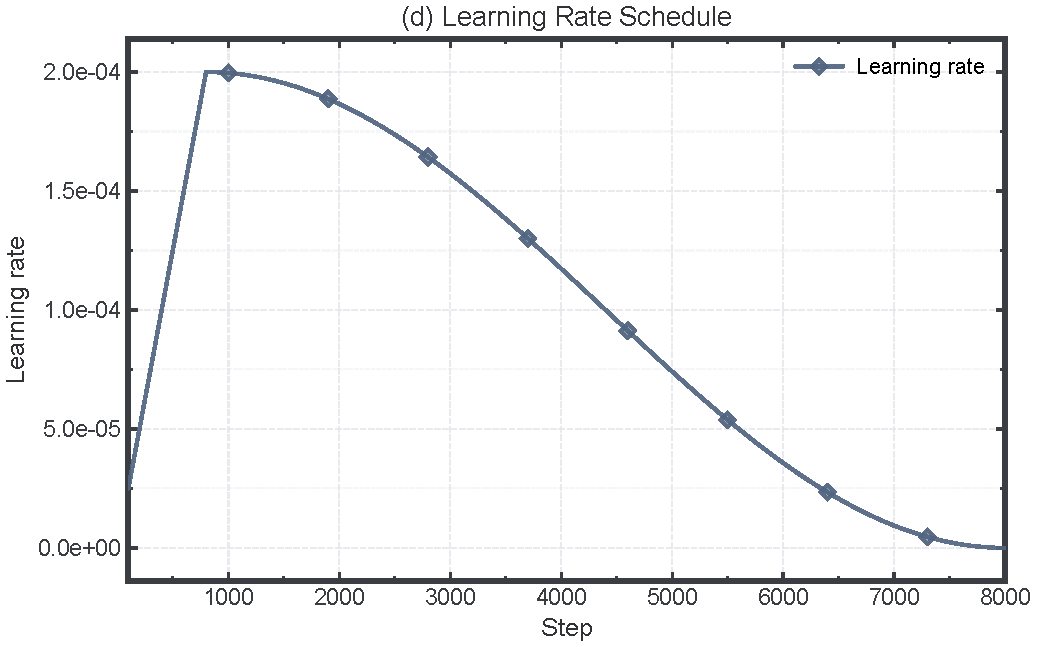
\includegraphics[width=\linewidth]{../sample_llm_training_curves_d_lr_schedule.pdf}
    \caption{Learning-rate schedule.}
  \end{subfigure}
  \caption{A full-width four-panel figure suitable for a paper's training
  analysis section. The panels share a common visual language while each
  remains legible at the final two-column width.}
  \label{fig:full-width}
\end{figure*}

\end{document}
